\ifdefined\included
\else
\documentclass[a4paper,11pt,twoside]{StyleThese}
\usepackage{amsmath,amssymb}             % AMS Math
\usepackage[T1]{fontenc}
\usepackage[utf8x]{inputenc}
\usepackage{babel}
\usepackage{datetime}

\usepackage{lmodern}
\usepackage{tabularx}
%\usepackage{tabular}
\usepackage{multirow}

\usepackage{hhline}
\usepackage[left=1.5in,right=1.3in,top=1.1in,bottom=1.1in,includefoot,includehead,headheight=13.6pt]{geometry}
\renewcommand{\baselinestretch}{1.05}

% Table of contents for each chapter

\usepackage[nottoc, notlof, notlot]{tocbibind}
\usepackage{minitoc}
\setcounter{minitocdepth}{2}
\mtcindent=15pt
% Use \minitoc where to put a table of contents

\usepackage{aecompl}

% Glossary / list of abbreviations

\usepackage[intoc]{nomencl}
\iftoggle{ThesisInEnglish}{%
\renewcommand{\nomname}{Glossary}
}{ %
\renewcommand{\nomname}{Liste des Abréviations}
}

\makenomenclature

% My pdf code

\usepackage{ifpdf}

\ifpdf
  \usepackage[pdftex]{graphicx}
  \DeclareGraphicsExtensions{.jpg}
  \usepackage[a4paper,pagebackref,hyperindex=true]{hyperref}
  \usepackage{tikz}
  \usetikzlibrary{arrows,shapes,calc}
\else
  \usepackage{graphicx}
  \DeclareGraphicsExtensions{.ps,.eps}
  \usepackage[a4paper,dvipdfm,pagebackref,hyperindex=true]{hyperref}
\fi

\graphicspath{{.}{images/}}

%% nicer backref links. NOTE: The flag ThesisInEnglish is used to define the
% language in the back references. Read more about it in These.tex

\iftoggle{ThesisInEnglish}{%
\renewcommand*{\backref}[1]{}
\renewcommand*{\backrefalt}[4]{%
\ifcase #1 %
(Not cited.)%
\or
(Cited in page~#2.)%
\else
(Cited in pages~#2.)%
\fi}
\renewcommand*{\backrefsep}{, }
\renewcommand*{\backreftwosep}{ and~}
\renewcommand*{\backreflastsep}{ and~}
}{%
\renewcommand*{\backref}[1]{}
\renewcommand*{\backrefalt}[4]{%
\ifcase #1 %
(Non cité.)%
\or
(Cité en page~#2.)%
\else
(Cité en pages~#2.)%
\fi}
\renewcommand*{\backrefsep}{, }
\renewcommand*{\backreftwosep}{ et~}
\renewcommand*{\backreflastsep}{ et~}
}

% Links in pdf
\usepackage{color}
\definecolor{linkcol}{rgb}{0,0,0.4} 
\definecolor{citecol}{rgb}{0.5,0,0} 
\definecolor{linkcol}{rgb}{0,0,0} 
\definecolor{citecol}{rgb}{0,0,0}
% Change this to change the informations included in the pdf file

\hypersetup
{
bookmarksopen=true,
pdftitle="Évaluation de la sécurité des équipements grand public connectés à Internet",
pdfauthor="Yann BACHY", %auteur du document
pdfsubject="Thèse", %sujet du document
%pdftoolbar=false, %barre d'outils non visible
pdfmenubar=true, %barre de menu visible
pdfhighlight=/O, %effet d'un clic sur un lien hypertexte
colorlinks=true, %couleurs sur les liens hypertextes
pdfpagemode=None, %aucun mode de page
pdfpagelayout=SinglePage, %ouverture en simple page
pdffitwindow=true, %pages ouvertes entierement dans toute la fenetre
linkcolor=linkcol, %couleur des liens hypertextes internes
citecolor=citecol, %couleur des liens pour les citations
urlcolor=linkcol %couleur des liens pour les url
}

% definitions.
% -------------------

\setcounter{secnumdepth}{3}
\setcounter{tocdepth}{2}

% Some useful commands and shortcut for maths:  partial derivative and stuff

\newcommand{\pd}[2]{\frac{\partial #1}{\partial #2}}
\def\abs{\operatorname{abs}}
\def\argmax{\operatornamewithlimits{arg\,max}}
\def\argmin{\operatornamewithlimits{arg\,min}}
\def\diag{\operatorname{Diag}}
\newcommand{\eqRef}[1]{(\ref{#1})}

\usepackage{rotating}                    % Sideways of figures & tables
%\usepackage{bibunits}
%\usepackage[sectionbib]{chapterbib}          % Cross-reference package (Natural BiB)
%\usepackage{natbib}                  % Put References at the end of each chapter
                                         % Do not put 'sectionbib' option here.
                                         % Sectionbib option in 'natbib' will do.
\usepackage{fancyhdr}                    % Fancy Header and Footer

% \usepackage{txfonts}                     % Public Times New Roman text & math font
  
%%% Fancy Header %%%%%%%%%%%%%%%%%%%%%%%%%%%%%%%%%%%%%%%%%%%%%%%%%%%%%%%%%%%%%%%%%%
% Fancy Header Style Options

\pagestyle{fancy}                       % Sets fancy header and footer
\fancyfoot{}                            % Delete current footer settings

%\renewcommand{\chaptermark}[1]{         % Lower Case Chapter marker style
%  \markboth{\chaptername\ \thechapter.\ #1}}{}} %

%\renewcommand{\sectionmark}[1]{         % Lower case Section marker style
%  \markright{\thesection.\ #1}}         %

\fancyhead[LE,RO]{\bfseries\thepage}    % Page number (boldface) in left on even
% pages and right on odd pages
\fancyhead[RE]{\bfseries\nouppercase{\leftmark}}      % Chapter in the right on even pages
\fancyhead[LO]{\bfseries\nouppercase{\rightmark}}     % Section in the left on odd pages

\let\headruleORIG\headrule
\renewcommand{\headrule}{\color{black} \headruleORIG}
\renewcommand{\headrulewidth}{1.0pt}
\usepackage{colortbl}
\arrayrulecolor{black}

\fancypagestyle{plain}{
  \fancyhead{}
  \fancyfoot{}
  \renewcommand{\headrulewidth}{0pt}
}

%\usepackage{MyAlgorithm}
%\usepackage[noend]{MyAlgorithmic}
\usepackage[ED=MITT - STICRT, Ets=INSA]{tlsflyleaf}
%%% Clear Header %%%%%%%%%%%%%%%%%%%%%%%%%%%%%%%%%%%%%%%%%%%%%%%%%%%%%%%%%%%%%%%%%%
% Clear Header Style on the Last Empty Odd pages
\makeatletter

\def\cleardoublepage{\clearpage\if@twoside \ifodd\c@page\else%
  \hbox{}%
  \thispagestyle{empty}%              % Empty header styles
  \newpage%
  \if@twocolumn\hbox{}\newpage\fi\fi\fi}

\makeatother
 
%%%%%%%%%%%%%%%%%%%%%%%%%%%%%%%%%%%%%%%%%%%%%%%%%%%%%%%%%%%%%%%%%%%%%%%%%%%%%%% 
% Prints your review date and 'Draft Version' (From Josullvn, CS, CMU)
\newcommand{\reviewtimetoday}[2]{\special{!userdict begin
    /bop-hook{gsave 20 710 translate 45 rotate 0.8 setgray
      /Times-Roman findfont 12 scalefont setfont 0 0   moveto (#1) show
      0 -12 moveto (#2) show grestore}def end}}
% You can turn on or off this option.
% \reviewtimetoday{\today}{Draft Version}
%%%%%%%%%%%%%%%%%%%%%%%%%%%%%%%%%%%%%%%%%%%%%%%%%%%%%%%%%%%%%%%%%%%%%%%%%%%%%%% 

\newenvironment{maxime}[1]
{
\vspace*{0cm}
\hfill
\begin{minipage}{0.5\textwidth}%
%\rule[0.5ex]{\textwidth}{0.1mm}\\%
\hrulefill $\:$ {\bf #1}\\
%\vspace*{-0.25cm}
\it 
}%
{%

\hrulefill
\vspace*{0.5cm}%
\end{minipage}
}

\let\minitocORIG\minitoc
\renewcommand{\minitoc}{\minitocORIG \vspace{1.5em}}

\usepackage{multirow}
%\usepackage{slashbox}

\newenvironment{bulletList}%
{ \begin{list}%
	{$\bullet$}%
	{\setlength{\labelwidth}{25pt}%
	 \setlength{\leftmargin}{30pt}%
	 \setlength{\itemsep}{\parsep}}}%
{ \end{list} }

\newtheorem{definition}{Définition}
\renewcommand{\epsilon}{\varepsilon}

% centered page environment

\newenvironment{vcenterpage}
{\newpage\vspace*{\fill}\thispagestyle{empty}\renewcommand{\headrulewidth}{0pt}}
{\vspace*{\fill}}

\usepackage{tablefootnote}

\usepackage{hyperref}
\hypersetup{
     colorlinks   = true,
     citecolor    = violet
}
\usepackage{graphicx} % for pdf, bitmapped graphics files
\usepackage{amsmath} % assumes amsmath package installed
\usepackage{amssymb}  % assumes amsmath package installed
\usepackage{bm} % for using bold lowercase greek letters
\usepackage{array}
\usepackage{colortbl}	% to color table background
%\usepackage[table]{xcolor}
\usepackage{subfigure}  
\usepackage{tikz}
\newcommand{\tikzcircle}[2][red,fill=red]{\tikz[baseline=-0.5ex]\draw[#1,radius=#2] (0,0) circle ;}%
\definecolor{turquoise}{rgb}{0.28 1 0.92}
\newcommand{\fratop}[2]{\genfrac{}{}{0pt}{}{#1}{#2}}
\newcommand{\mx}[1]{\mathbf{\bm{#1}}} 				% Matrix symbol
\newcommand{\vc}[1]{\mathbf{\bm{#1}}} 					% Vector symbol
\newcommand{\degree}{\ensuremath{^\circ}}				% define the degree symbol
\newcommand{\pder}[2]{\frac{\partial#1}{\partial#2}}		% partial derivative
\newcommand{\ppder}[2]{\frac{\partial^2 #1}{\partial#2^2}}		% second partial derivative
\newcommand{\refframe}[1]{\mbox{\textless#1\textgreater}}	% to denote a reference frame
%\DeclareMathOperator*{\lexmin}{\text{lex}\!\min}			% lexmin
\DeclareMathOperator*{\minimize}{minimize}				% minimize
\DeclareMathOperator*{\maximize}{maximize}				% maximize
%\DeclareMathOperator*{\argmin}{\arg\!\min}				% argmin
%\DeclareMathOperator*{\argmax}{\arg\!\max}				% argmax
\DeclareMathOperator*{\st}{subject\,to}					% subject to
\DeclareMathOperator*{\dif}{\mathrm{d}}					% d
\DeclareMathOperator*{\half}{\frac{1}{2}}					% one half
\newcommand{\mat}[1]{\ensuremath{\begin{bmatrix}#1\end{bmatrix}}}	% matrix
\newcommand{\rank}[1]{\text{rank}(#1)}							% rank
%\newcommand{\diag}[1]{\text{diag}(#1)}							% diag
\newcommand{\x}{\ensuremath{\times}}
\newcommand{\spac}{\ensuremath{\quad}}						% alias for space in math environment
\newcommand{\dt}[0]{\ensuremath{\Delta t}}					% dt
\newcommand{\dx}[0]{\ensuremath{\delta x}}					% dx
\newcommand{\du}[0]{\ensuremath{\delta u}}					% du
\newcommand{\dhu}[0]{\ensuremath{\delta \hat{u}}}					% \hat{du}
\newcommand{\dbu}[0]{\ensuremath{\delta \bar{u}}}					% \bar{du}
\newcommand{\dtu}[0]{\ensuremath{\delta \tilde{u}}}					% \tilde{du}
\newcommand{\dhx}[0]{\ensuremath{\delta \hat{x}}}					% \hat{dx}
\newcommand{\DX}[0]{\ensuremath{\Delta X}}						% DX
\newcommand{\DU}[0]{\ensuremath{\Delta U}}						% DU
\newcommand{\Ts}[0]{\ensuremath{\top}}							% transpose symbol
\newcommand{\pinv}[0]{\ensuremath{\dagger}}					% pseudoinverse symbol
\newcommand{\Rv}[1]{\ensuremath{\mathbb{R}^{#1}}}				% set of real-valued vectors
\newcommand{\Rm}[2]{\ensuremath{\mathbb{R}^{#1\times #2}}}		% set of real-valued matrices
\newcommand{\Spd}[1]{\ensuremath{\mathbb{S}_+^{#1}}}			% set of symmetric positive-definite matrices
\newcommand{\card}[1]{\ensuremath{\left\vert{#1}\right\vert}}			% cardinality of a set
\DeclareMathOperator{\Tr}{Tr}							% trace
\newcommand{\Expect}{{\rm I\kern-.3em E}}				% expectation
\newcommand{\Normal}{\mathcal{N}}					% normal distribution
\newcommand{\Prob}[1]{\text{P}(#1)}						% probability
\newcommand{\vech}[1]{\text{vech}(#1)}						% vech

\newcommand{\sethree}{\ensuremath{SE(3)}}
\newcommand{\CS}{$\mathcal{CS}$}
\newcommand{\WS}{$\mathcal{WS}$}
\newcommand{\CSfree}{$\mathcal{CS}_{free}$}
\newcommand{\CSobst}{$\mathcal{CS}_{obst}$}
\newcommand{\M}[0]{$\mathcal{M}$}

%\algnewcommand{\algorithmicgoto}{\textbf{go to}}%
%%\algnewcommand{\Goto}[1]{\algorithmicgoto~\ref{#1}}%
%\algnewcommand{\Goto}{\algorithmicgoto\xspace}%
%\algnewcommand{\Label}{\State\unskip}

\newenvironment{definition}[1][Definition]{\begin{trivlist}
\item[\hskip \labelsep {\bfseries #1}]}{\end{trivlist}}

\usepackage{epstopdf}
\usepackage[colorinlistoftodos,prependcaption,textsize=tiny]{todonotes}
\newcommand\explainmore[1]{\textcolor{red}{#1}}
\newcommand\refrephrase[1]{\textcolor{yellow}{#1}}
\newcommand\donerephrasing[1]{\textcolor{green}{#1}}

%DIF PREAMBLE EXTENSION ADDED BY LATEXDIFF
%DIF UNDERLINE PREAMBLE %DIF PREAMBLE
\RequirePackage[normalem]{ulem} %DIF PREAMBLE
\RequirePackage{color}\definecolor{RED}{rgb}{1,0,0}\definecolor{BLUE}{rgb}{0,0,1} %DIF PREAMBLE
\providecommand{\DIFadd}[1]{{\protect\color{blue}\uwave{#1}}} %DIF PREAMBLE
\providecommand{\DIFdel}[1]{{\protect\color{red}\sout{#1}}}                      %DIF PREAMBLE
%DIF SAFE PREAMBLE %DIF PREAMBLE
\providecommand{\DIFaddbegin}{} %DIF PREAMBLE
\providecommand{\DIFaddend}{} %DIF PREAMBLE
\providecommand{\DIFdelbegin}{} %DIF PREAMBLE
\providecommand{\DIFdelend}{} %DIF PREAMBLE
%DIF FLOATSAFE PREAMBLE %DIF PREAMBLE
\providecommand{\DIFaddFL}[1]{\DIFadd{#1}} %DIF PREAMBLE
\providecommand{\DIFdelFL}[1]{\DIFdel{#1}} %DIF PREAMBLE
\providecommand{\DIFaddbeginFL}{} %DIF PREAMBLE
\providecommand{\DIFaddendFL}{} %DIF PREAMBLE
\providecommand{\DIFdelbeginFL}{} %DIF PREAMBLE
\providecommand{\DIFdelendFL}{} %DIF PREAMBLE
%DIF END PREAMBLE EXTENSION ADDED BY LATEXDIFF


\begin{document}


\sloppy
\begin{document}
\setcounter{chapter}{1} %% Numéro du chapitre précédent ;)
\dominitoc
\faketableofcontents
\fi

\chapter{Robustness to Inertial Parameter Errors for Legged Robots Balancing on Level Ground}
\label{chapter:rc}
% \section{Abstract}
% Model-based control  has become more and more popular in the legged robots community in the last ten years. 
% The key idea is to exploit a model of the system to compute precise motor commands that result in the desired motion.
% This allows to improve the quality of the motion tracking, while using lower gains, leading so to higher compliance.
% However, the main flaw of this approach is typically its lack of robustness to modeling errors.
% In this paper we focus on the robustness of inverse-dynamics control to errors in the inertial parameters of the robot.
% We assume these parameters to be known, but only with a certain accuracy.
% We then propose a computationally-efficient optimization-based controller that ensures the balance of the robot despite these uncertainties.
% We used the proposed controller in simulation to perform different reaching tasks with the HRP-2 humanoid robot, in the presence of various modeling errors.
% Comparisons against a standard inverse-dynamics controller through hundreds of simulations show the superiority of the proposed controller in ensuring the robot balance.


Model-based control has become more and more popular in the legged robots community in the last ten years. 
The key idea is to exploit a model of the system to compute precise motor commands that result in the desired motion.
This allows to improve the quality of the motion tracking, while using lower gains, leading so to higher compliance.
However, the main flaw of this approach is typically its lack of robustness to modeling errors. In this chapter we focus on the robustness of inverse-dynamics control to errors in the inertial parameters of the robot. We assume these parameters to be known, but only with a certain accuracy. We then propose a computationally-efficient optimization-based controller that ensures the balance of the robot despite these uncertainties. We used the proposed controller in simulation to perform different reaching tasks with the HRP-2 humanoid robot, in the presence of various modeling errors.Comparisons against a standard inverse-dynamics controller through hundreds of simulations show the superiority of the proposed controller in ensuring the robot balance.
\section{Introduction}
The problem of balancing for real legged robots is still a challenge for the robotics community.
Although our understanding of this problem has remarkably improved during the last 15 years, the robustness of the state-of-the-art control algorithms is far from satisfactory.
For instance, during the recent DARPA Robotics Challenge Finals~\cite{Pratt2015}, all legged robots have moved extremely cautiously, and, despite that, sometimes they could not avoid falling.
Another striking fact is the difference between what robots can do in simulation where they easily perform extremely dynamics tasks and what they can do in the real world where they struggle to execute slow movements in structured environments.
The gap between simulation and real world can be explained through countless unmodeled uncertainties affecting these systems, such as poor torque control, model uncertainties, sensor noises and delays.
In recent work of ~\cite{DelPrete2015b}, an optimization-based controller tries to ensure the satisfaction of the physical constraints of the robot (force friction cones, joint acceleration limits and torque limits) despite errors in the joint torque tracking. In this work we move along the same line, designing a \emph{robust} controller that can balance a legged robot despite bounded errors in its inertial parameters.




The chapter starts with a brief discussion about various control methodologies used in humanoid robots (Section~\ref{sec:control_methods}). Section~\ref{sec:soa_robust} presents robustness related work in optimization based control. In Section~\ref{sec:tsid} we model the uncertainty in the inertial parameters of the robot through polytopes. Then we present the Task-Space Inverse Dynamics(TSID) controller with capture-point constraints~\cite{Ramos2014a} to ensure the balance of the robot in case of no modeling errors. Section~\ref{sec:robustness} presents an extension of the standard capture-point inequalities that is robust to errors in the inertial parameters.We first formulate the associated robust optimization problem, and then use standard robust-optimization techniques to reformulate it in a tractable form. (Section~\ref{sec:tests}) presents statistical results that compare in simulation the standard and the robust controller in a reaching task with the humanoid robot HRP-2. Regardless of the simulation conditions, our results empirically demonstrate the superiority of the proposed robust controller with respect to standard TSID. Finally, Section~\ref{sec:conclusions} draws the conclusions and discusses the future work.



\section{Robustness in Humanoid Robots}
\label{sec:soa_robust}
Even though the problem of robustness is long-standing and well-identified, it remains largely unanswered for legged robots. 
Some approaches focus exclusively on the stability of the system rather than on the feasibility of the trajectories.
For instance, adaptive control~\cite{Kelly1989} and time-delay estimation~\cite{Jin2008} try to estimate and compensate online for the major errors between nominal and real dynamic model.
Virtual model control~\cite{Pratt} does not rely on the dynamic model of the robot, which ensures robustness to errors in the inertial parameters~\cite{dietrich2013multi}. 
The main issue of these schemes is that they do not consider inequality constraints, which makes it hard to implement them on real systems, given the large number of bounds to which they are subject.

Other approaches are based on hand-tunable heuristics. For instance, a common heuristic in Task-Space Inverse Dynamics (TSID)~\cite{DelPrete2014c} which we adopt as well is to use a secondary task to keep the robot posture close to a reference one, in order to keep the movements far from the joint limits. 
Similarly, to avoid slipping/tipping, it was proposed to minimize the contact moments and the tangential contact forces in the null space of the main motion task~\cite{Righetti2010}. 
Yet another common trick during locomotion is to maintain the center of pressure close to the center of the foot~\cite{Kajita2003}.
The robotics literature is filled with these kinds of heuristics, which often are the main reason behind the successful implementations on real platforms.
However, these heuristics can not ensure feasibility in the presence of any significant uncertainty and needs ad-hoc tuning depending on the situation.

Finally, another class of works which includes this work makes use of robust optimization techniques to formulate control and planning problems.
Mordatch et al.~\cite{Mordatch2015} considered several perturbed models of a humanoid robot to plan offline a trajectory that is robust to uncertainties, reporting success rate between 80\% and 95\% on a real platform. 
Another recent work~\cite{Luo} has combined robust and time-scaling optimization to plan trajectories that are robust to bounded errors in friction coefficients and joint accelerations, whose magnitude can be estimated online through iterative learning.
Nguyen and Sreenath~\cite{Nguyen} have recently exploited control Lyapunov functions and Quadratic Programs (QPs) to ensure stability despite bounded uncertainties in the linearized system dynamics. 

Contrary to~\cite{Mordatch2015,Nguyen}, the uncertainties modeled in this work affect the parameters of the system, so they could be identified using set-membership identification techniques~\cite{Ramdani2005}.
The main contribution in this work is a novel formulation of the capture-point balance constraints, which can be included in the Task-Space Inverse Dynamics optimization problem to balance the robot despite bounded uncertainties in its inertial parameters.
Contrary to previous approaches that dealt with uncertainties to inertial parameters, our approach allows us to include inequality constraints in the problem formulation.
Thanks to this we can thus account for all the constraints to which legged robots are subject, ensuring the feasibility of the resulting trajectories.


\section{Task-Space Inverse Dynamics with Capture-Point Balance Constraints}
\label{sec:tsid}
To design a controller that is robust to errors in the inertial parameters of the robot we have first to understand how these errors affect the control action.
In this section we define the inertial parameters and we present a standard Task-Space Inverse Dynamics controller, which includes balance constraints. 
Throughout the presentation we explicitly show the dependency of the terms on the inertial parameters, while we omit the dependency on the robot configuration $q$ and velocities $v$ because they are constant values at each time step.

\subsection{Inertial Parameters}
We define the vector containing the 10 inertial parameters of link $i$ as:
\begin{equation*}
\phi_i = (m_i, m_i {}^i c_i, I_i^{xx}, I_i^{xy}, I_i^{xz}, I_i^{yy}, I_i^{yz}, I_i^{zz} ),
\end{equation*}
where $m_i \in \Rv{}$ is the mass, $c_i \in \Rv{3}$ is the CoM, $I_i \in \Rm{3}{3}$ is the 3D rotational inertia matrix.
Both $c_i$ and $I_i$ are expressed in the local reference frame of the link.
Note that $\phi_i$ does not contain directly $c_i$, but it contains only its product with $m_i$.
This is because the robot dynamics can be written in a linear form with respect to this parameterization of the inertial parameters~\cite{Traversaro2015}.

Now we can collect the inertial parameters of all the $N$ links of the robot in a single vector:
\begin{equation*}
\phi = (\phi_1, \dots, \phi_N)
\end{equation*}
We assume that each link parameters $\phi_i$ are not known exactly, but we know that they lie inside a polytope $U_i$, i.e. $\phi_i \in U_i$.
Hence also the vector $\phi$ lies inside a polytope:
$$
\phi \in U = U_1 \times \dots \times U_N
$$
Note that since a polytope can be represented by a set of linear inequalities, the constraint $\phi_i \in U_i$ can be expressed under the form $A_i \phi_i \le a_i$. Now that we defined the inertial parameters and the associated uncertainty polytopes, we can see how these uncertainties affect the controller.
\subsection{Task-Space Inverse Dynamics}
The controller that we consider in this work is an optimization-based inverse dynamics controller, which computes the desired torques taking into account the dynamcis of the robot. It has become a standard for the control of legged robots in recent years~\cite{DelPrete2014c,Herzog2016,Sentis2004,Saab2011}. Table \ref{table:simu_params} shows TSID outperforming other control frameworks.
Theortically, the kinematics and dynamics are decoupled. Kinematic level task prioritization is done first to compute acceleration and the torques are calculated to achieve the computed accelerations. 
\begin{table}[bh] 
\caption{Comparison of Control Frameworks\cite{DelPrete2014c}}
\centering 
\begin{tabular}{|p{3.5cm} | p{1.2cm} p{1.2cm} p{1.2cm} p{1.2cm} p{1.4cm} p{1.1cm}|}
\hline 
	Framework		& Optimal & Efficient & Force& Under & Inequality & Output \\ 
 	& & & Control & actuated& &  \\ \rowcolor[gray]{.9}   
\hline 
	TSID\cite{DelPrete2014c}& $\times$ & $\times$ & $\times$ & $\times$ & & $\tau$ \\
	UF\cite{Peters2007}		&  & $\times$ & $\times$ &  & & $\tau$ \\  \rowcolor[gray]{.9}
	WBCF\cite{Sentis2005}	& $\times$ &  & $\times$ & $(\times)$ &  & $\tau$\\ 
	\cite{Mistry2011}		&  & & $\times$ & $\times$ & & $\tau$ \\ \rowcolor[gray]{.9}
	SoT\cite{Saab2011}		& $\times$ &  & $\times$ & $\times$ & $\times$& $\tau$ \\  
	\cite{DeLasa2009}		& $\times$ & &$\times$& $\times$ &  & $\tau$ \\  \rowcolor[gray]{.9}
	\cite{Jeong2009}		& $\times$ & $\times$ &  &  & & $\tau/\ddot{q}$ \\      
	\cite{nakamura1987task}		& & $\times$ &  &  & & $\dot{q}/\ddot{q}$ \\ \rowcolor[gray]{.9}
    	\cite{Chiaverini1997}		& & $\times$ &  &  & & $\dot{q}$ \\ 
	\cite{siciliano1991general}	& $\times$ & $\times$ &  &  & & $\dot{q}$ \\  \rowcolor[gray]{.9}

	\cite{Baerlocher1998}		& $\times$ & $\times$ &  &  & & $\dot{q}$ \\  
	\cite{Smits2008}		& $\times$ & $\times$ &  &  & $\times$& $\dot{q}$ \\   \rowcolor[gray]{.9}        
%	$K_p^{reach}$ 	& Reaching proportional gain 	& $20-80$ \\ \rowcolor[gray]{.9}
%	$K_p^{post}$ 	& Posture proportional gain 	& $20$ \\
[0.5ex] \hline 
\end{tabular} 
\label{table:simu_params} %\bigskip
\end{table}
% \explainmore{The generic method proposed in this thesis is based on the inverse-dynamics model of the robot considering contact constraints and a set of tasks specified with a given priority. The resolution for each task is posed as a minimization problem, subject to several constraints that ensure dynamic feasibility, and uses a hierarchical scheme based on hierarchized QPs. Since the motion is generated using several prioritized tasks, and the dynamic model of the robot is taken into account, the term Dynamic Stack of Tasks (SoT) is sometimes used to refer to the framework. With respect to other operational-space inversedynamics (OSID) approaches, the advantages of the proposed method are the capability to handle both equality and inequality constraints at any level of the hierarchy, the fast computation time that allows it execution in real-time, and the direct feasibility of the generated motion, which does not need any further processing or validation before being executed on the robot.}
Various formulations of the TSID optimization problem exist and are often equivalent or similar~\cite{DelPrete2014c}.
We write it here as an optimization problem of the base and joint accelerations $\dot{v} \in \Rv{n+6}$, the contact forces \mbox{$f\in \Rv{k}$}, and the joint torques $\tau \in \Rv{n}$~\cite{Saab2013}:
\begin{subequations} 
\label{eq:TSID}
\begin{align}
\minimize_{y=(\dot{v}, f, \tau)} \quad &|| A y - a||^2 \nonumber\\
\st \quad & \mat{M(\phi) & -J_c^\TS & -S^\TS \\ J_c & 0 & 0} \mat{\dot{v} \\ f \\ \tau} = \mat{- h(\phi) \\ -\dot{J}_c v} \nonumber\\
& | \tau | \le \tau^{max} \label{eq:TSID_torque_lim}\\
& \dot{v}^{min} \le \dot{v} \le \dot{v}^{max} \label{eq:TSID_acc_lim}\\
& f \in \mathcal{K} \label{eq:TSID_force_lim}
\end{align} 
\end{subequations}
where \mbox{$J_c \in \Rm{k}{(n+6)}$} is the constraint Jacobian, $M \in \Rm{(n+6)}{(n+6)}$ is the mass matrix, $h \in \Rv{n+6}$ contains the bias forces, $S\in \Rm{n}{(n+6)}$ is the selection matrix, $\tau^{max} \in \Rv{n}$ are the maximum joint torques, $\dot{v}^{min/max} \in \Rv{n+6}$ are the acceleration bounds\footnote{The bounds of the joint positions and velocities are typically converted into joint-acceleration bounds~\cite{Padois2010}}, and $\mathcal{K}$ is the force friction cone (which is typically linearized).
The cost function represents the error of the task, which is typically an affine function of $\dot{v}$ (i.e. a task-space acceleration):
\begin{equation*} \begin{aligned}
\underbrace{\mat{J_{task} & 0 & 0}}_A y - \underbrace{(\ddot{x}_{task}^{des} - \dot{J}_{task} v)}_a = \ddot{x}_{task} - \ddot{x}_{task}^{des}
\end{aligned} \end{equation*}
The task may be to track a predefined trajectory of a link, of the CoM of the robot, or to regulate the robot angular momentum.

\subsection{Capture Point}
Regardless of the task they are performing, legged robots must take care of balancing (i.e. avoiding to fall) at the same time.
Balancing is fundamental for legged robots and it has been extensively studied~\cite{Collette2008,Morisawa2012,Goswami2004,Hyon2006,Sherikov}.
This problem is particularly well understood for robots in contact with a flat terrain only.
In this case, the dynamics of the robot CoM $c$ is well approximated by a linear inverted pendulum.
In this model the robot is approximated as a point mass (maintained at a constant height) supported by a variable-length leg link~\cite{Pratt2006}.
The resulting dynamics is:
\begin{equation*}
\ddot{c}^{xy}(\phi) = \omega(\phi)^2 (c^{xy}(\phi) - u),
\end{equation*}
where $u \in \Rv{2}$ is the ZMP, which is equivalent to the center of pressure~\cite{Wieber2002}, and \mbox{$\omega(\phi) = \sqrt{\frac{g}{c^z(\phi)}}$}.
The same dynamics can also be obtained from the real dynamics of the robot CoM, by assuming that $\dot{c}^z=0$ and the rate of change of the robot angular momentum is null~\cite{Wieber}.
Using this linear dynamics we can compute the point on the ground where the robot can put its ZMP to in order to stop its CoM:
\begin{equation*}
\xi(\phi) = c^{xy}(\phi) + \frac{\dot{c}^{xy}(\phi)}{\omega(\phi)}
\end{equation*}
This point is known as the capture point~\cite{Pratt2006}, the divergent component of motion or the extrapolated CoM ~\cite{Wieber}.

\subsection{Capture-Point Balance Constraints}
Originally, the capture point was used to decide where to make the robot step in order to recover from a push~\cite{Pratt2006}.
More recently, Ramos et al.~\cite{Ramos2014a} proposed use it to ensure the balance of the robot.
The key idea is that, as long as the capture point remains inside the convex hull of the contact points (i.e. the so-called \emph{support polygon} $\mathcal{S}$), the robot can balance without taking a step. 
To ensure the balance of the robot we can then add to \eqref{eq:TSID} another set of inequalities to constrain the capture point to remain inside the support polygone:
$$
B (\xi(\phi) + \dt \dot{\xi}(\phi))  \le b,
$$
where $\dot{\xi}(\phi) \in \Rv{2}$ is the time derivative of the capture point, and the matrix $B$ and the vector $b$ define the support polygon (i.e. $B x \le b \Longleftrightarrow x \in \mathcal{S}$).
By expressing $\xi$ and its derivative as functions of $c^{xy}$ and its derivatives we get:
\begin{align*}
B \left ( c^{xy}(\phi) + \frac{\dot{c}^{xy}(\phi)}{\omega(\phi)} + \dt \left( \dot{c}^{xy}(\phi) + \frac{\ddot{c}^{xy}(\phi)}{\omega(\phi)} \right) \right)  \le b \\
B \left ( c^{xy}(\phi) + \alpha(\phi) \dot{c}^{xy}(\phi) + \frac{\dt}{\omega(\phi)} \ddot{c}^{xy}(\phi) \right)  \le b,
\end{align*}
where $\alpha(\phi) = \dt + \omega(\phi)^{-1}$.
Finally we can express the CoM acceleration $\ddot{c}^{xy}$ as a function of the joint accelerations $\dot{v}$:
\begin{equation} \label{eq:cp_ineq}
D(\phi) \dot{v} + B \left (c^{xy}(\phi) + \alpha(\phi) \dot{c}^{xy}(\phi) + \beta(\phi) \right ) \le b,
\end{equation}
where: 
\begin{align*}
D(\phi) &= \frac{\dt}{\omega(\phi)} B J_{com}(\phi) \\
\beta(\phi) &= \frac{\dt}{\omega(\phi)} \dot{J}_{com}(\phi) v
\end{align*}
These inequalities are linear with respect to the joint accelerations $\dot{v}$, so they can be added to the QP problem \eqref{eq:TSID} to ensure the robot balance in case of no modeling uncertainties.



\section{Robustness to Inertial Parameter Errors}
\label{sec:robustness}
In the previous section we saw that the inertial parameters appear in three different locations in the controller optimization problem \eqref{eq:TSID}: i) in the mass matrix $M$, ii) in the bias forces $h$, and iii) in the capture-point inequalities \eqref{eq:cp_ineq}.
Unfortunately $M$ and $h$ depend on $\phi$ in a highly-nonlinear way, so it is hard to deal with it.
In this work we deal instead with the dependency of the capture-point inequalities \eqref{eq:cp_ineq} on the inertial parameters.
More in details, many terms in \eqref{eq:cp_ineq} depend on $\phi$, but we will focus on the dependency of the CoM xy coordinates on $\phi$.
In other words, we want to solve this optimization problem:
\begin{subequations} 
\label{eq:rob_TSID}
\begin{align} 
\minimize_{y=(\dot{v}, f, \tau)} \quad &|| A y - a||^2 \nonumber \\
\st \quad & \mat{M(\hat{\phi}) & -J_c^\T & -S^\T \\ J_c & 0 & 0} \mat{\dot{v} \\ f \\ \tau} = \mat{- h(\hat{\phi}) \\ -\dot{J}_c v} \\
& \eqref{eq:TSID_torque_lim}, \eqref{eq:TSID_acc_lim}, \eqref{eq:TSID_force_lim} \nonumber \\
& D(\hat{\phi}) \dot{v} + B c^{xy}(\phi) \le \bar{b}(\hat{\phi}) \quad \forall \phi \in U, \label{eq:rob_TSID_cp}
\end{align} 
\end{subequations}
where $\hat{\phi}$ are the nominal inertial parameters (i.e. those used by the standard controller) and:
$$
\bar{b}(\hat{\phi}) = b - B (\alpha(\hat{\phi}) \dot{c}^{xy}(\hat{\phi}) + \beta(\hat{\phi}))
$$
Problem \eqref{eq:rob_TSID} is not tractable because it has an infinite number of inequality constraints due to the capture-point inequalities that need to be satisfied for all the possible values of $\phi$.
In order to solve \eqref{eq:rob_TSID} we need to reformulate it in a tractable form.
To do that, we will start by analyzing the relationship between $c^{xy}$ and $\phi$ (which is linear).
Then we will show how to reformulate the robust capture-point inequalities \eqref{eq:rob_TSID_cp} in a tractable form.

\subsection{Dependency of CoM on Inertial Parameters}
The CoM of the robot is the average of the CoM of all its links, weighted by their respective masses:
\begin{equation} \label{eq:com} \begin{aligned}
c^{xy} &= P \frac{ \sum_{i=1}^{N} m_i (p_i + {}^wR_i {}^ic_i) }{m_{tot}} \\
       &= \sum_{i=1}^{N} \underbrace{m_{tot}^{-1} P \mat{p_i & {}^wR_i & 0_{3\times 6}}}_{F_i} \phi_i \\
       &= \mat{F_1 & \dots & F_N} \phi = F \phi,
\end{aligned} \end{equation}
where  $P= {\tiny\mat{1&0&0\\0&1&0}}$, $p_i \in \Rv{3}$ is the position of the reference frame of link $i$ expressed in the world frame, ${}^wR_i \in \R{3}{3}$ is a rotation matrix from link $i$ reference frame to the world frame, and $m_{tot}$ is the total mass of the robot.
From \eqref{eq:com} we can see that the robot CoM is the ratio of two linear functions of the inertial parameters because $m_{tot}$ is clearly a linear function of $\phi$.
However, given that we can easily know the robot total mass, we can assume that the uncertainty in $m_{tot}$ be negligible.
In the context of robustness we can thus consider $c^{xy}$ as a linear function of $\phi$.

\subsection{Robust Capture-Point Inequalities}
Now we want to reformulate the robust capture-point inequalities into a tractable form.
We can start by rewriting the $i$-th line of \eqref{eq:rob_TSID_cp} using \eqref{eq:com}:
\begin{align*}
D_i \dot{v} + B_i F \phi \le \bar{b}_i \qquad \forall \phi \in U,
\end{align*}
where $D_i, B_i$ and $\bar{b}_i$ are the $i$-th lines of the associated matrix/vector, and we dropped the dependency on the nominal inertial parameters $\hat{\phi}$ for the sake of readability.
We can get rid of the quantifier operator $\forall$ by replacing the uncertain term with its maximum:
\begin{align}
D_i \dot{v} + \max_{\phi \in U} (B_i F \phi) \le \bar{b}_i
\end{align}
We could compute the maximum of $B_i G \phi$ under the constraint of $\phi$ belonging to the polytope $U$ by solving a Linear Program (LP) for each capture-point inequality.
However, that would be too computationally expensive for a controller that typically has to run at 1 kHz because of the size of the LP (i.e. $10N$ variables and even more constraints).
Luckily we show now that we can solve this LP by solving $N$ LPs of much smaller size.
\begin{align}
\max_{\phi \in U}  B_i F \phi = \max_{\phi \in U}  \sum_{j=1}^N B_i F_j \phi_j = 
\sum_{j=1}^N \max_{\phi_j \in U_j} B_i F_j \phi_j
\end{align}
Thanks to this reformulation, rather than maximizing a linear function of the robot CoM, we can maximize a linear function of each link CoM.
This boils down to finding, for each link, the CoM position that maximizes the dot product with the vector $B_i$.
If the polytope of possible CoM positions has not many vertices, this optimization can be performed by enumeration.
This means that we can compute the dot product of $B_i$ with all the vertices of the CoM polytope and then take the one that resulted in the largest value.
Since the vertices of the CoM polytope of each link can be computed offline before starting the controller, this operation is extremely computationally efficient.
If we assume that each CoM polytope has $n_v$ vertices and that the support polygone has $n_s$ sides, the computation of $\max_{\phi \in U}  B_i F \phi$ for all  $i$ requires $n_s n_v N$ dot products of 3D vectors.
For a typical scenario of $n_s=6$, $n_v=10$ and $N=30$, this gives 1800 dot products.
On a standard computer this would take only a few microseconds, so it is suitable for real-time control on a real robot.

Once this quantity has been computed, the robust capture-point inequalities \eqref{eq:rob_TSID_cp} can be written as standard linear inequalities and problem \eqref{eq:rob_TSID} can be solved by a standard QP solver.



\section{Tests}
\label{sec:tests}
In this section, we present a series of simulation results that try to answer to the following question: what improvement can we get in terms of fall prevention by using the robust controller?
We tested the proposed controller on a typical humanoid tasks (i.e. whole-body reaching) with the 30-degree-of-freedom humanoid robot HRP-2.
We carried out several batches of tests, each batch differing for the simulated uncertainties. 
Each batch was composed by 100 tests, which is not enough for being a statistically significant sampling, but was dictated by the computation time of our simulation environment (about 6 hours for 100 tests).
Each test consisted in trying to perform the reaching motion with the two controllers (classic and robust) until the robot either fell or reached the end of the motion.
The inertial parameter errors changed at each test, but they were the same for the two controllers.
We then measured the number of times each controller drove the robot to a fall and the average distance between the final end-effector position and the desired target.

\subsection{Simulation Environment}
\begin{table}[!tbp] 
\caption{Simulation parameters.}
\centering 
\begin{tabular}{p{1.1cm} | p{3.8cm} p{1.8cm}}
\hline 
	Symbol		& Meaning 				& Value \\ \rowcolor[gray]{.9}
\hline 
	$\dt$			& Simulation time step 		& 0.002 s \\
	$\dot{v}_j^{max}$ & Max joint acceleration		& $10 \, \text{rad} \, \text{s}^{-2}$ \\ \rowcolor[gray]{.9}
	$v_j^{max}$	& Max joint velocity			& $9.14 \, \text{rad} \, \text{s}^{-1}$ \\
	$\mu$		& Force friction coefficient		& 0.3 \\  \rowcolor[gray]{.9}
	$w_{reach}$	& Reaching weight 		& $1$ \\ 
	$w_{post}$ 	& Posture weight 			& $10^{-2}$ \\ \rowcolor[gray]{.9}
	$w_{force}$ & Force minimization weight 			& $10^{-5}$ \\ 
%	$K_p^{reach}$ 	& Reaching proportional gain 	& $20-80$ \\ \rowcolor[gray]{.9}
%	$K_p^{post}$ 	& Posture proportional gain 	& $20$ \\
[0.5ex] \hline 
\end{tabular} 
\label{table:simu_params} %\bigskip
\end{table}
To assess the proposed controller we developed a dedicated simulation environment based on a state-of-the-art algorithm for frictional contacts in multibody systems~\cite{Kaufman2008}. 
We integrated the equations of motion of the system with a first-order Euler scheme with fixed time step $\dt$.
Our choice of not using an off-the-shelf simulator is motivated by our desire to completely understand and control the simulation environment. 
The inertial parameters (masses and centers of mass) of the model used by the controller did not match those of the model used by the simulator. 
The random inertial-parameter errors were generated using uniform distribution. 
For masses, the maximum error was expressed in terms of percentage of the real values. 
For centers of mass, the maximum error was instead expressed in meters. 
In each test we specify which uncertainties were simulated. 
Table~\ref{table:simu_params} lists all the simulation and controller parameters.

\subsection{Task Description}
The control objective was defined by three tasks that the robot had to perform at the same time. 
Since the tasks are in conflict, we weighted them with hand-tuned parameters, according to their importance.
The three tasks, in order of decreasing priority, are:
\begin{itemize}
\item reach the desired target with the right end-effector (weight $w_{reach}$)
\item maintain initial joint posture (weight $w_{post}$)
\item minimize contact moments and tangential forces~\cite{Righetti2013} (weight $w_{force}$)
\end{itemize}


We carried out two sets of simulations.
In both cases HRP-2 executed a reaching motion that made its capture point reach the boundaries of its support polygon. 


\begin{figure*}[!tbph]
\centering
\begin{subfigure}
[Classic control illustrating the robot's loss of balance when the real capture point gets out of the support polygon]{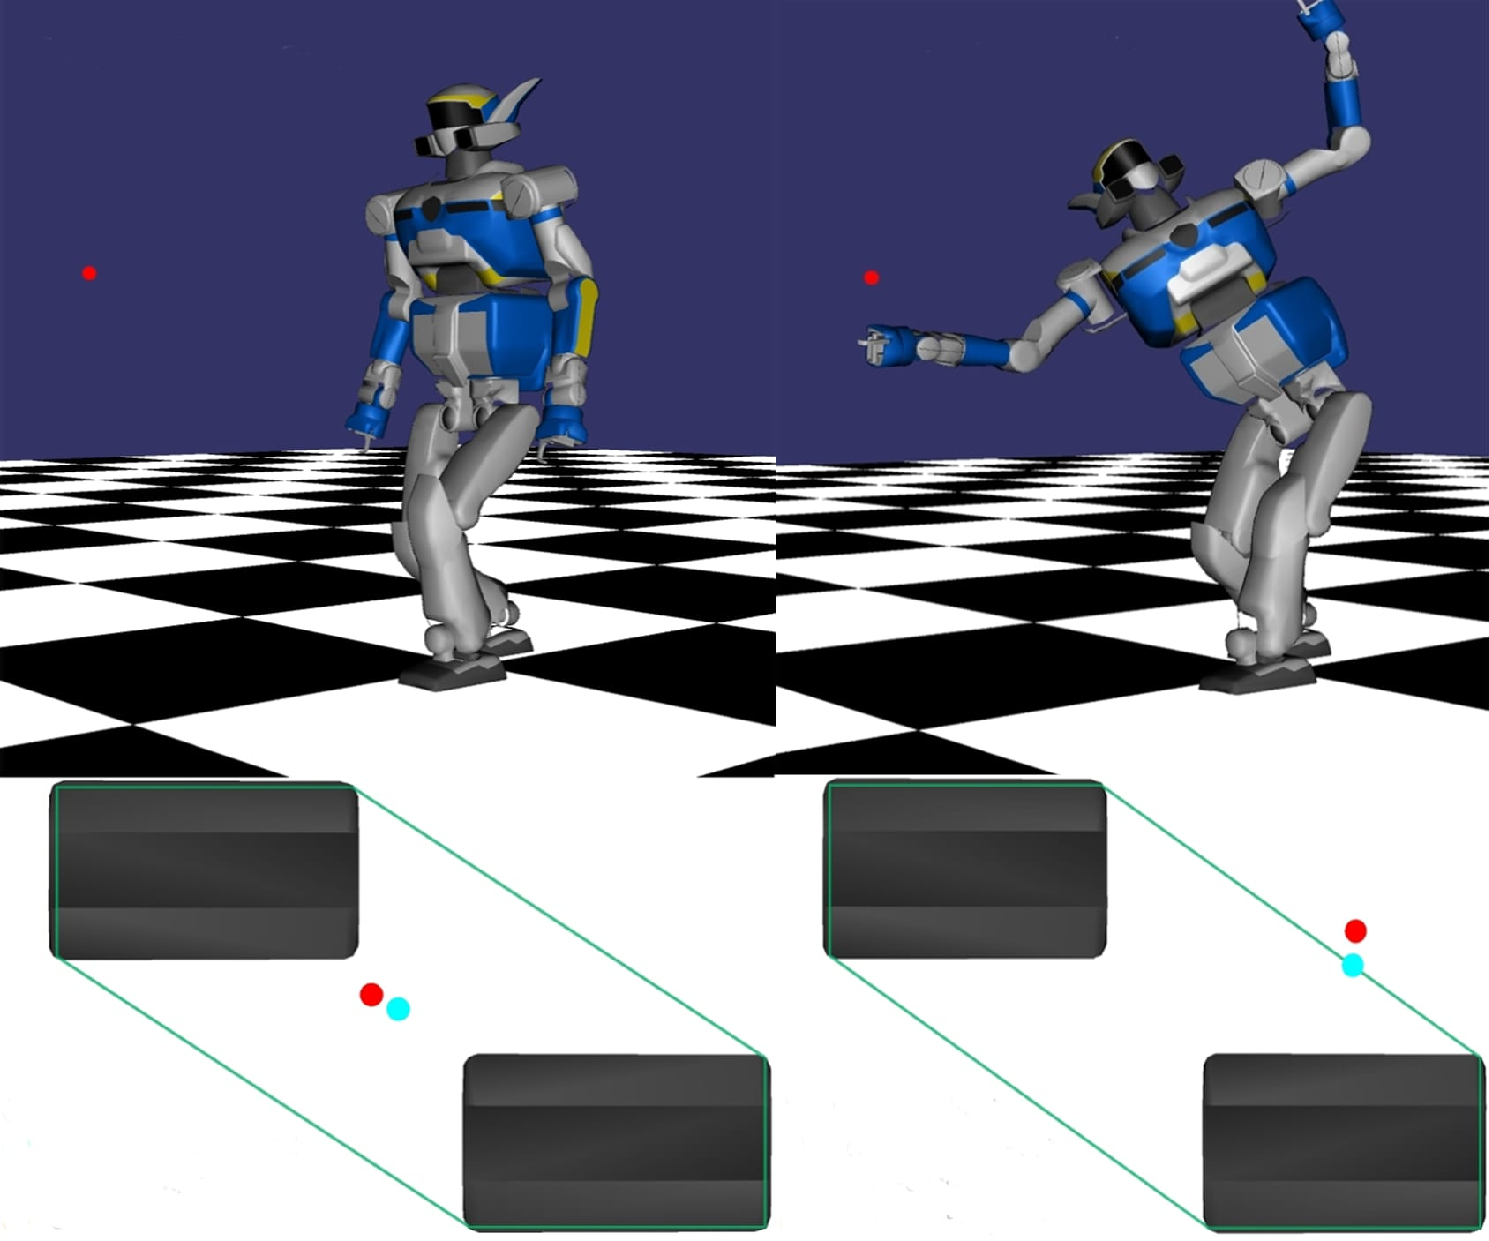
\includegraphics[scale=0.4]{rc_inertial_params/classic_merge.pdf}}\quad
\end{subfigure}
\begin{subfigure}
[Robust control illustrating the robot right end effector reaching close to the goal without losing balance]{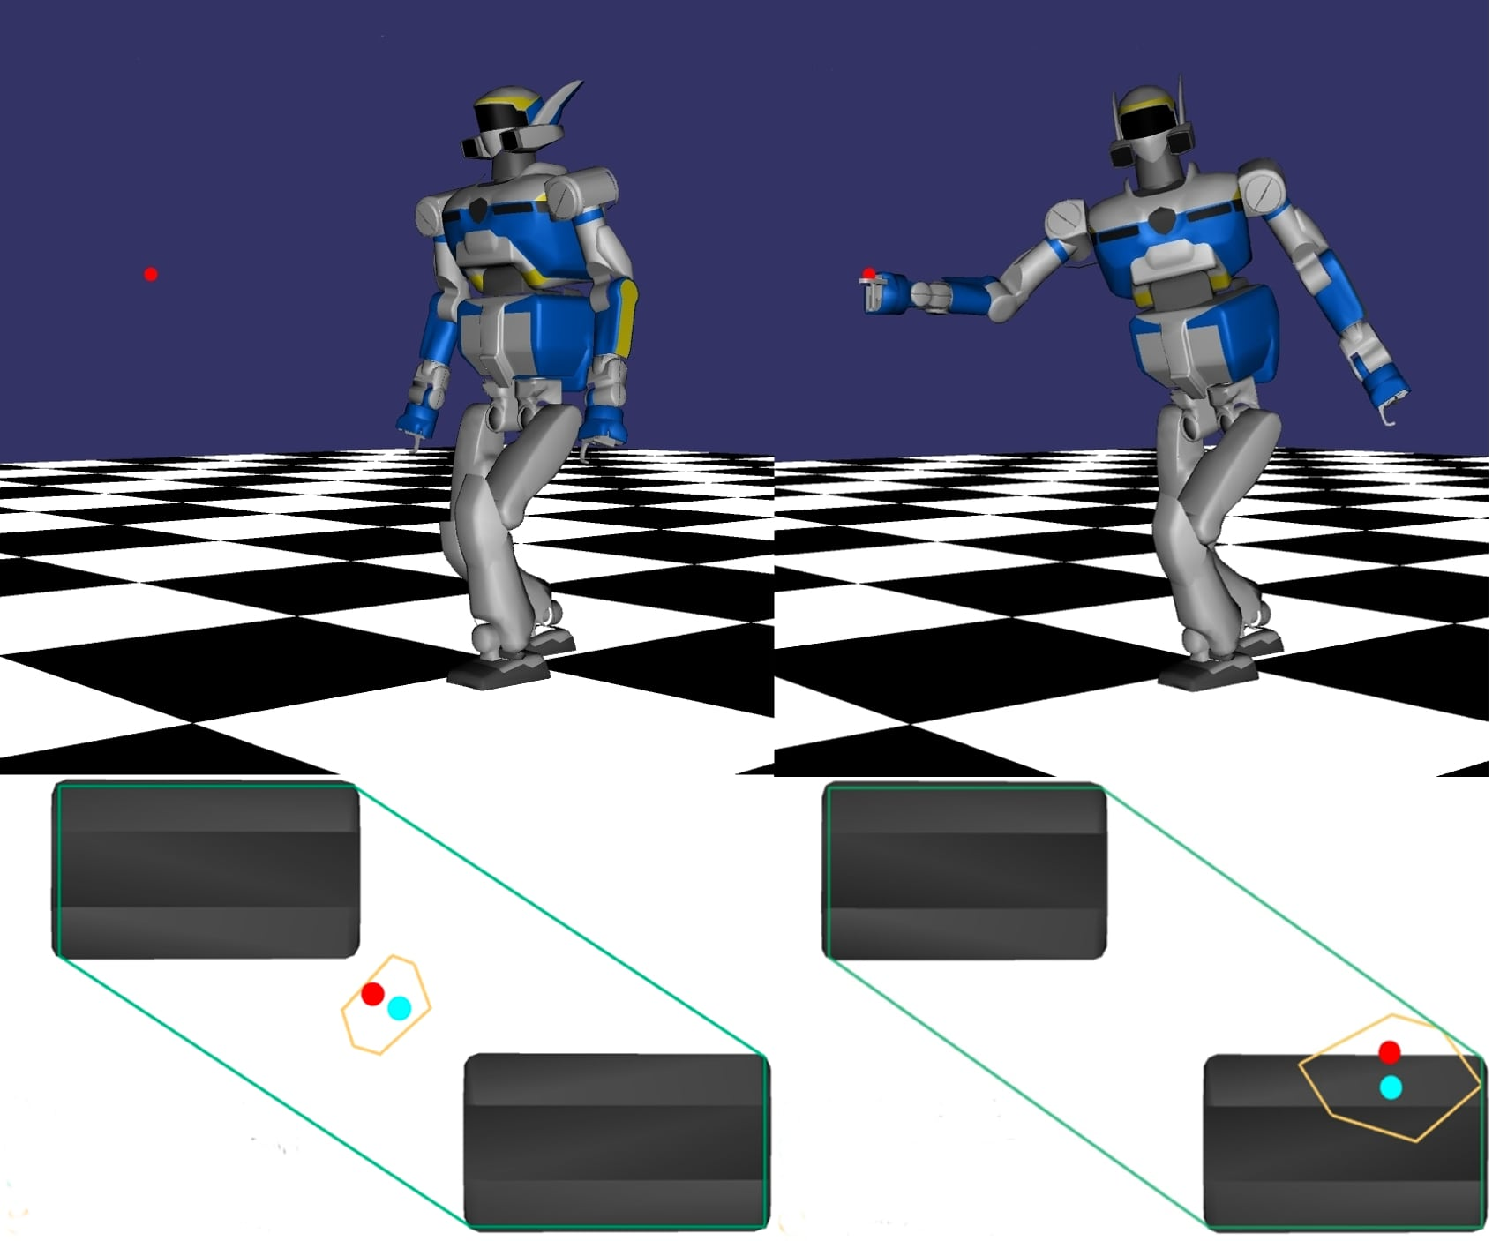
\includegraphics[scale=0.4]{rc_inertial_params/robust_merge.pdf}}\quad
\end{subfigure}\\
 \tikzcircle{3pt}  \footnotesize Real Capture Point \tikzcircle[turquoise, fill=turquoise]{3pt} Estimated Capture Point   \tikzcircle[green, fill=green]{3pt} Support Polygon   \tikzcircle[yellow, fill=yellow]{3pt} Capture Point Polytope

\caption{Screenshots of HRP-2 executing Test 1 to reach the ball target with the robust controller.}
\label{fig:control}
\end{figure*}


\begin{table*}[!tbph]
\begin{center}
\caption{Results of Test 1. For each controller we show the number of falls (Falls), the average time to complete the motion (Task Time) and the average distance of the end-effector to the target at the end of the motion (Task Error).}
\begin{tabular}{ |l|l|l|l|l|l|l|l| }
\hline
\multicolumn{2}{|c|}{Uncertainties}&\multicolumn{3}{|c|}{Classic Controller}&\multicolumn{3}{|c|}{Robust Controller}\\
\hline Max Mass & Max CoM &{Falls}& Task &{Task} & Falls & Task& Task  \\
Error & Error & & Time   &  Error & &  Time & Error\\ 
{[\%]} & [mm] & [\%]  &  [s]  &  [mm]  & [\%]  &  [s] & [mm]\\ 
\hline
% 10 & 12.5& 35& 6.22&4& 1& 5.26& 5\\
% 10 & 25  & 31 & 6.30&  5& 0& 7.32& 12\\
% 10 & 50  & 43 & 4.49 & 70 & 0 & 4.66 & 110\\
% 30 & 50  & 43 & 4.48 & 70 & 0 & 4.68 & 110\\
% 30 & 100 & 40 & 5.44 & 30 & 4 & 5.81 & 80 \\
10 & 10 & 31 & 4.4 & 49 & 3 & 4.5 & 60\\
10 & 20 & 33 & 4.3 & 52 & 1 & 4.5 & 69 \\
10 & 40 & 45 & 4.3 & 55 & 3 & 4.7 & 102\\ 
20 & 10 & 38 & 4.2 & 49 & 11 & 4.5 & 77\\
20 & 20 & 49 & 4.5 & 51 & 9 & 4.55 & 103 \\
20 & 40 & 45 & 4.5 & 59 & 14 & 4.72 & 122 \\
\hline
\end{tabular}
\label{tab:test1}
\end{center}
\end{table*}
\subsection{Test 1}
In this test we set the right end-effector target far in front of the robot.
Fig.~\ref{fig:control}  shows some screen shots of the simulations.
To reach the target the robot must move its CoM (and hence also its capture point) close to the boundaries of its support polygon. 
Table~\ref{tab:test1} presents the results. 
Regardless of the magnitude of the inertial parameter errors, the robust controller managed to prevent the robot from falling almost always, while with the  standard controller the robot fell more than 30\% of the times.
However, since the target was far away from the robot, the robust controller did not manage to reach it because that would have required violating the robust balance constraints.
\begin{table*}[!h]
\begin{center}
\caption{Results of Test 2. For each controller we show the number of falls (Falls), the average time to complete the motion (Task Time) and the average distance of the end-effector to the target at the end of the motion (Task Error).}
\begin{tabular}{ |l|l|l|l|l|l|l|l| }
\hline Max Mass & Max CoM &{Falls}& Task &{Task} & Falls & Task& Task  \\
Error & Error & & Time   &  Error & &  Time & Error\\ 
{[\%]} & [mm] & [\%]  &  [s]  &  [mm]  & [\%]  &  [s] & [mm]\\ 
\hline
% 10 & 12.5 & 59 & 3.64& 0 & 5 & 3.06& 0\\
% 10 & 25.0 & 42 & 3.40 & 0.18 & 4 & 2.94 & 0.12 \\
10 & 10 & 29 & 3.94 & 2 & 0 & 3.4 & 2 \\
10 & 20 & 35 & 3.4 & 2 & 2 & 3.0 & 2 \\
10 & 40 & 42 & 3.86 & 4 & 0 & 2.6 & 4 \\
20 & 10 & 43 & 3.6 & 3 & 0 & 2.8 & 4 \\
20 & 20 & 45 & 3.5 & 3 & 0 & 2.5 & 4 \\
20 & 40 & 45 & 3.0 & 5 & 0 & 2.1 & 5 \\

\hline
\end{tabular}
\label{tab:test2}
\end{center}
\end{table*}
\subsection{Test 2}
In this test we moved the right end-effector target closer to the robot, so that HRP-2 can reach it without moving its CoM close to the support polygon boundaries.
However, we increased the desired speed of reaching (by increasing the gains of the reaching task).
This affected the velocity of the CoM, which in turns affected the capture point, making it reach the boundaries of the support polygon.
The difference with respect to Test 1 is that in this case also the robust controller can reach the target.
Table~\ref{tab:test2} summarizes the results.

Similarly to Test 1, the classic controller leads the robot to a fall in more than 30\% of the cases.
However, contrary to Test 1, this time the robust controller also manages to reach the target, because it is located closer to the robot.
This test shows that being robust does not necessarily implies that we have to sacrifice performance. A video result of the same is available \href{https://youtu.be/IA-HhoR0g-4}{\textcolor{blue}{here}}.



%!TEX root =  ../root.tex
\section{Conclusions}
\label{sec:conclusions}
This chapter presented a novel optimization-based inverse-dynamics controller that can balance a legged robot despite bounded uncertainties in its inertial parameters. The controller is based on the state-or-the-art control framework Task-Space Inverse Dynamics. In particular, this work is based on the capture-point inequalities~\cite{Ramos2014a}, which can be included in the controller formulation to ensure the balance of the robot on a level ground. We extended these capture-point inequalities to be robust to bounded uncertainties in the inertial parameters of the robot. The resulting optimization problem is still a Quadratic Program with the same number of variables and inequalities. Moreover, the time required for the additional computation of the robust controller is negligible in this context (i.e. a few microseconds).

We tested the robust controller in simulations with the HRP-2 robot, trying to reach a target position with its right end-effector while balancing. We performed several batches of 100 simulations each, introducing different errors in the inertial parameters and varying the position of the target position and the required speed of motion. Comparisons against a classic TSID controller have shown impressive improvements in terms of fall prevention.


